\setcounter{section}{5}
\phantomsection
\section*{Data and Methodology}
\addcontentsline{toc}{section}{Data and Methodology}

In this section, we explain the data sources used in the analytical process, how the main variables were constructed and then describe our empirical strategy. The dataset consists of European scholars that include family relationships, academic careers, multiple measures of productivity and recognition, biographical traits and regional inheritance systems. The empirical approach takes advantage of within-family variation between brothers to estimate birth-order effects controlling for unobserved family-level characteristics.

\phantomsection
\subsection*{3.1 Data Sources}
\addcontentsline{toc}{subsection}{3.1 Data Sources}

The dataset is constructed using the Repertorium Eruditorum Totius Europae (RETE) database, which provides standardized biographical information on European scholars and is based on a wide range of historical sources \citep{curtis2026academic}. At the individual level, this includes year of birth and death, place of birth, and detailed records of academic activities and careers.

This secondary source is complemented with information drawn directly from primary historical sources, including published biographical repertories of university professors (e.g. the Italian Repertorio dei professori for institutions such as the University of Bologna ), which provide structured individual entries and often include information on family relationships, such as fathers and siblings. These sources are used to identify and complete family links between individuals.

Academic productivity is measured using bibliometric indicators derived from the Virtual International Authority File (VIAF) and related catalogues. These sources aggregate information from national libraries and authority files to identify publications associated with each individual, allowing the construction of indicators such as the number of titles, publishers, publication countries, coauthors, and works with ISBN identifiers \citep{curtis2026academic}.

In addition, encyclopedic recognition is proxied using Wikipedia-based measures, including the length of articles and the number of languages in which an individual is represented. Data on academic careers are further refined using records of institutional affiliations over time, which enable the identification of each scholar’s primary institution and the construction of measures such as the number of affiliations over the career.

Taken together, these sources provide a detailed and multifaceted perspective on long-run scholarly productivity and recognition.

\phantomsection
\subsection*{3.2 Construction of Brother Pairs}
\addcontentsline{toc}{subsection}{3.2 Construction of Brother Pairs}
 
Two complementary sources are identified by brother pairs. When a direct information on brothers in the secondary source or in a biographical dictionary is available, we use it. Second, we construct additional brother pairs by locating fathers with multiple sons in the academic records. For each father with minimum 2 sons, all posssible pairs of brothers are created.

To avoid duplication, brother pairs are treated as unordered pairs and duplicates are removed. Pairs in which both siblings refer to the same individual are excluded. Birth order is determined using year-of-birth information. A pair is classified as \emph{rankable} if birth years are known for both brothers and differ across siblings, allowing the identification of the older and younger brother. Pairs for which birth years are missing or identical are classified as \emph{unrankable}.

The primary analytical sample is 619 pairs of brothers with identifiable birth order which can be ranked. Unrankable pairs are preserved for the purposes of a description and analysis of sample composition over time. Table~\ref{tab:descriptives} presents descriptive statistics for the analytical sample.

There is considerable variation in age gaps between brothers in the historical data with a non-negligible share of pairs having large spacing. To distinguish birth-order effects from cohort and life-cycle differences, the empirical analysis explicitly controls for age gaps. Figure~\ref{fig:age_gap} shows the distribution of the age gaps.

\phantomsection
\subsection*{3.3 Outcome Variables}
\addcontentsline{toc}{subsection}{3.3 Outcome Variables}
 
The primary outcomes of interest reflect academic productivity and recognition. Metrics indicating productivity are: the number of titles attributed to an individual in bibliographic records or counts of publishers, publishing countries, coauthors and publications with ISBN numbers. As these variables are highly skewed with a high number of zero outcomes, the main analysis uses inverse hyperbolic sine transformations.

Recognition is measured using Wikipedia-based indicators, such as how long an individual’s Wikipedia page is and in how many languages there may be an entry. These measures include visibility and perceived importance in the historical narrative, in addition to bibliographic productivity indicators.

By assigning outcomes independently to the older and younger brother for rankable pairs, we make direct within-family comparisons possible. Table~\ref{tab:ttests} presents the outcome of paired comparison analyses across all dependent measures.

\phantomsection
\subsection*{3.4 Temporal Assignment and Century Classification}
\addcontentsline{toc}{subsection}{3.4 Temporal Assignment and Century Classification}

Each brother pair is assigned a reference period to study long-run patterns and historical composition. If the birth years of both siblings are known, then the reference year is defined as the average between two birth years. If only one birth year is observed, that birth year is used directly to assign the corresponding century.

For missing birth years, the analysis is based on academic entry dates contructed from when recorded academic activities started. For these cases, academic entry years are translated into approximate birth years by subtracting from the respective academic entry year an estimate corresponding to the average age at which individuals entered academia within our sample of rankable pairs which is 34.86 years. Appendix Figure~\ref{fig:age_entry} shows the distribution of entry ages in the sample.

And while unrankable pairs occur throughout the sample, most observations correspond to rankable pairs for which we can identify birth order. Figure~\ref{fig:rankable_century} depicts how many of the brother pairs fall into the rankable vs unrankable bins, sorted by century. The number of pairs of brothers rises sharply in the later centuries, which reflects the greater availability and completeness of historical records closer to the modern period.

\begin{figure}[htbp]
\centering
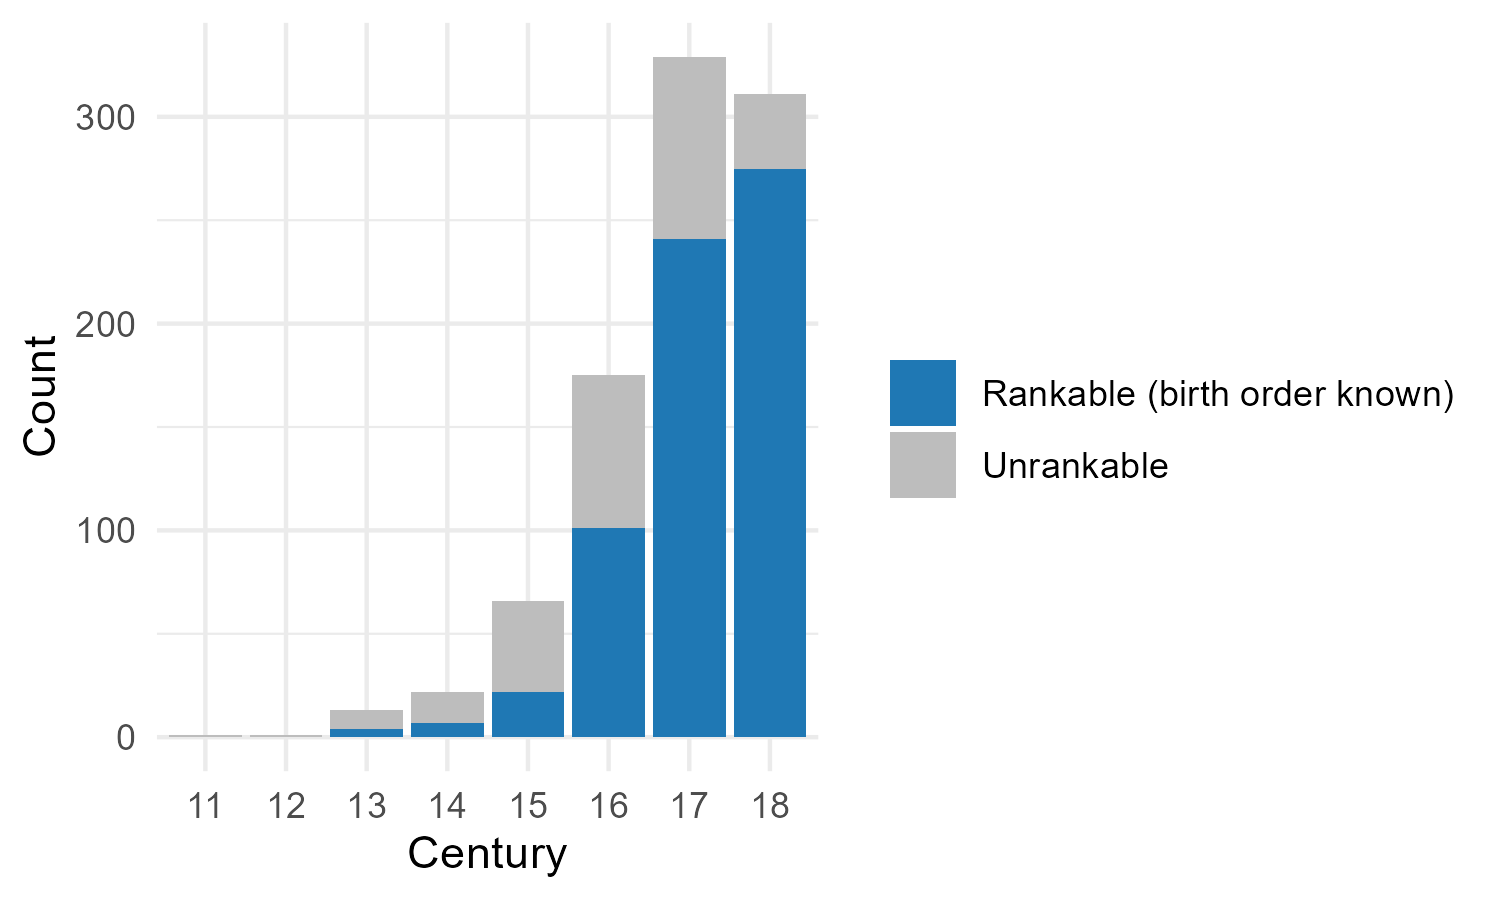
\includegraphics[width=0.8\textwidth]{figures/Plot_Rankable_vs_Unrankable.png}
\caption{Rankable and Unrankable Brother Pairs by Century}
\label{fig:rankable_century}
\begin{minipage}{0.85\textwidth}
\footnotesize
\textit{Notes:} The figure displays the number of brother pairs in the dataset by century, distinguishing between rankable pairs (for which birth order can be identified) and unrankable pairs (for which birth order cannot be determined due to missing or identical birth years).
\end{minipage}

\end{figure}
\FloatBarrier

\phantomsection
\subsection*{3.5 Inheritance Systems}
\addcontentsline{toc}{subsection}{3.5 Inheritance Systems}

In order to account for institutional variation between regions, the analysis includes information on inheritance systems according to the classification developed by \cite{Todd1990}. Regions are set up according to the predominant inheritance regime: primogeniture vs. egalitarian systems. For France we adapted the classification from \cite{Gobbi2024}.

We assign an inheritance system to each scholar based on their birthplace using a geographic mapping at the NUTS3 level. For brother pairs, if the birth order is known, we associate inheritance system indicators with the birthplace of the older brother. In Figure~\ref{fig:todd_map}, we provide a geographic visualization of inheritance systems and scholars’ birthplaces.

Because inheritance regimes affected incentives for parental investment and the expected returns from being the eldest son, the empirical strategy explicitly tests whether birth-order differentials in productivity differ across inheritance systems (primogeniture vs egalitarian). However, such comparisons only work for the oldest son; beyond that, they are not economically meaningful. Correspondingly, inheritance-driven dynamics limit attention to brother pairs that include the eldest son, aligning with the institutional logic of inheritance.

\phantomsection
\subsection*{3.6 Empirical Strategy}
\addcontentsline{toc}{subsection}{3.6 Empirical Strategy}

The empirical strategy leverages within-family variation for pairs of brothers. By comparing siblings within the same family, differences out many unobserved family-level characteristics that brothers may have in common, including parental background, socio-economic status and cultural environment. This within-family design thus enables us to isolate birth-order differences in scholarly outcomes.

All regression specifications cluster standard errors at the family level. Since brothers within the same household have common environments, parental background, and potentially correlated shocks to their academic trajectories, error terms can be correlated within-family. So clustering the standard errors at family level corrects this within-family correlation and makes sure our statistical inference is not misleadingly precise. Standard errors are family-clustered unless specified otherwise, for all regression-based results presented in the dissertation.

The analysis unfolds in stages. We first perform paired comparisons between older and younger brothers on multiple measures of scholarly productivity and recognition. These paired t-tests offer a transparency measure of whether systematic birth-order differences exist between families. Table~\ref{tab:ttests} reports on the outcomes of these comparisons.

Second, we examine whether the differences by birth order occur through extensive or intensive margins of scholarly activity. The extensive margin accounts for whether a scholar has any publications at all, and the intensive margin reflects productivity conditional on publishing. The extensive margin is estimated using a binary response model, whereas the intensive margin is estimated using OLS with an inverse hyperbolic sine transformation of titles. Both specifications control for age differences between siblings, and whether the father was active in academia. The results are presented in Table~\ref{tab:extensive_intensive}.

Third, we estimate regression models that directly assess the productivity gap between older and younger brothers while accounting for observable characteristics such as age gaps, family academic background, and institutional overlap. These specifications also include inheritance systems and temporal controls to investigate whether the birth-order effects are moderated by institutional environments and historical context. We present our main regression results in Table~\ref{tab:main_regressions}.

Finally, to evaluate the robustness of results, several checks are carried out. These cover limiting the sample to pairs with lower age differences, excluding families with greater than two sons, and estimating the regressions with other productivity variables (the length of the Wikipedia page, number of languages of the Wikipedia page, and number of publishers). The results are shown in Appendix Table~\ref{tab:robustness} and Table~\ref{tab:alt_measures}.

\phantomsection
\subsection*{3.7 Limitations}
\addcontentsline{toc}{subsection}{3.7 Limitations}
 
Several limitations should be noted. Firstly, historical data are incomplete and selective, since the sample comprises those who have left a trace in academic or bibliographic records. Secondly, birth years and family relationships may also be missing or inaccurate for some people. Third, measures of productivity only mirror output that is recorded and recognized rather than true underlying potential.

Nonetheless, the within-family approach, coupled with detailed biographical and institutional data, provides a powerful context for investigating birth-order effects on a elite population.